\chapter{Hardwareumsetzung}
\label{cha:robot}
\section{Entwurf des NXT-Roboters}

Die hardwareseitigen Voraussetzungen an den Roboter bestanden im Hauptsächlichen aus der freien Bewegung im Raum und dem Aufnehmen, Mitführen und Ablegen von kleinen Gegenständen in einem vordefinierten Bereich.

Nach kurzer Recherche\cite{building_instructions} und Durchsicht von Bauanleitungen für verschiedenste Anwendungsbereiche wurde sich für den Standardaufbau aus der zum Bauset zugehörigen LEGO NXT Bauanleitung entschieden.

Sie wurde lediglich um den Schall- und den Abstandssensor erleichtert; eine Halterung für das Smartphone wurde hinzugefügt.

\todo{hier Bild des Roboters einfügen}

\pagebreak

\subsection{Sensoren}

\subsubsection{Tastsensor}

\begin{figure}[h]
\centering
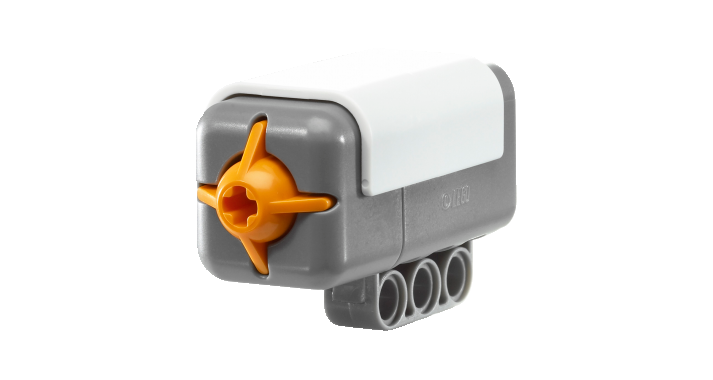
\includegraphics[width=\textwidth/3]{Bilder/Robot/button_sensor}
\caption{Tastsensor des NXT-Systems}
\label{fig:buttonSensor}
\end{figure}

Der berührungsempfindliche Sensor vorne diente zum Detektieren von Gegenständen im Bereich des Greifarms, woraufhin dieser geschlossen werden kann. Er wurde durch den Ultraschallsensor ersetzt, der nicht nur die unmittelbare Berührung bemerkt sondern auch ein herannahendes Objekt während der Fahrt detektiert.

\subsubsection{Rotationssensoren}

Die Rotationssensoren in den Servomotoren erlauben es dem NXT-Roboter, die Geschwindigkeit der Motoren abhängig des Widerstands (des Untergrunds) zu regulieren. So werden unter anderem präzises Abbremsen und Fehlerminimierung bei der Positionsbestimmung ermöglicht.

\subsubsection{Farbsensor}

\begin{figure}[h]
\centering
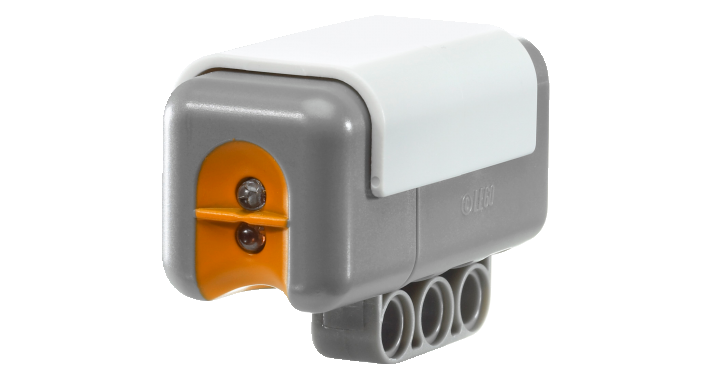
\includegraphics[width=\textwidth/3]{Bilder/Robot/color_sensor}
\caption{Farbsensor des NXT-Systems}
\label{fig:colorSensor}
\end{figure}

Der RGB-Sensor am Boden des NXT dient dazu, die Farbe des Bodens herauszufinden. Diese kann sowohl dazu genutzt werden, bei der Bildverarbeitung die Hintergrundfarbe herauszurechnen und so die Qualität der Objekterkennung zu erhöhen, als auch eine farblich markierte Zielzone im Raum finden zu können, auf der ein getragenes Objekt abgelegt werden kann.

\subsubsection{Ultraschallsensor}

\begin{figure}[h]
\centering
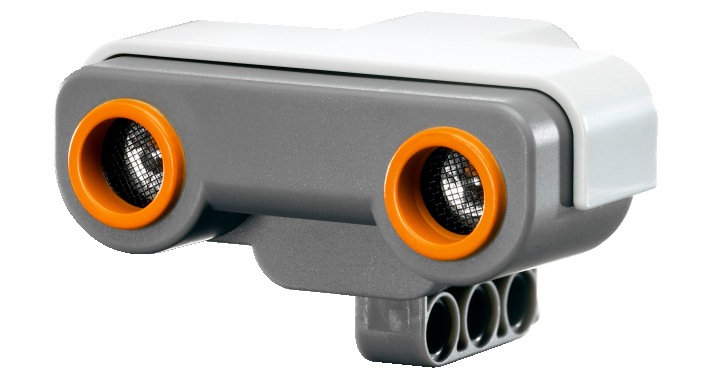
\includegraphics[width=\textwidth/3]{Bilder/Robot/distance_sensor}
\caption{Ultraschallsensor des NXT-Systems}
\label{fig:distanceSensor}
\end{figure}

Der Ultraschallsensor dient zur Messung der Distanz vom Roboter zum nächsten soliden Objekt. Hier wird er genutzt um zu detektieren, wie weit ein Objekt vom Greifarm entfernt ist, um diesen im geeigneten Moment zu schließen und so das Objekt mitnehmen zu können. Auch ermöglicht er ein geregeltes Heranfahren an ein Objekt. Die Präzision des Distanzsensors beträgt $\pm$3cm.

\subsection{Aktoren}

\subsubsection{Antriebsmotoren}

\begin{figure}[h]
\centering
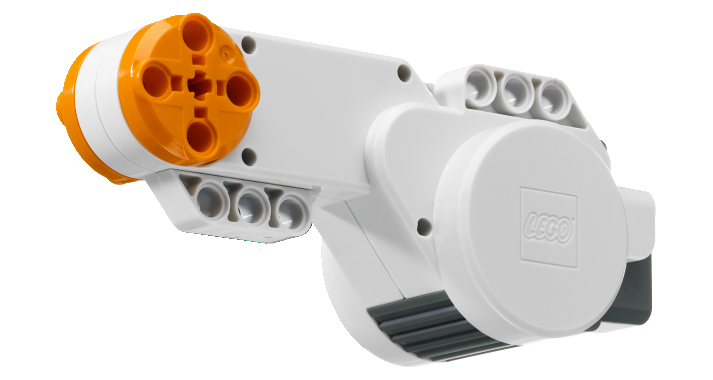
\includegraphics[width=\textwidth/3]{Bilder/Robot/motor}
\caption{Servo-Motor des NXT-Systems}
\label{fig:motor}
\end{figure}

Die beiden Servomotoren links und rechts des NXT-Roboters bilden den differentialen Antrieb und ermöglichen freie Fortbewegung.

\subsubsection{Greifarmmotor}
\label{greifarm}
Der dritte Motor im vorderen Teil des Roboters dient zum Öffnen und Schließen des Greifarms und so zur Mitführung von Gegenständen.

\section{Steuerung des Roboters}

Die Steuerung des Roboters durch das Smartphone erfolgt via Bluetooth.
Das Kommunikationsprotokoll und damit die nötigen Befehle zum Regeln der Aktoren und Auslesen der Sensoren wurde von LEGO dokumentiert und ist online erhältlich\cite{nxt_comm_protocol}.

Auf dem NXT selbst wird hierbei kein Programm ausgeführt, um alle Logik zentral in der NXT-App auf dem Smartphone zu halten.

Zunächst muss eine Bluetooth-Verbindung erstellt werden, wozu beide Geräte aktiviertes Bluetooth aufweisen, der Roboter zusätzlich sichtbar für das Smartphone sein müssen.

Bei Erstverbindung muss der gesuchte NXT ausgewählt werden, danach ist die Bluetooth-Adresse bekannt und die App kann ohne Benutzerinteraktion eine Verbindung mit dem NXT-Roboter aufnehmen.

Kommt eine Verbindung zustande, können seriell Byte für Byte die Kommandos an den NXT übertragen, eventuelle Antworten empfangen werden.

App-seitig übernimmt ein gesonderter Thread in der Klasse NxtTalker nach Zustandekommen einer Verbindung das Management der Daten.

Zum Bewegen der Motoren muss zunächst per Befehl pro Aktor eine Geschwindigkeit (und Parameter wie Regulierung) übergeben, zum Stoppen können alle Motoren mit einem Befehl auf Geschwindigkeit '0' gesetzt werden.

Zwei Motoren können synchronisiert werden, sodass diese gleichzeitig starten. Ansonsten würde der Zeitversatz zwischen dem Absetzen der zwei 'setze Geschwindigkeit'-Befehle bewirken, dass der Roboter vor dem geradeaus fahren kurz nur das erste Rad ansteuert und in eine Richtung abdriftet.

\section{Wahl des Kameramoduls}
\label{sec:Kamera}

Die Hauptfrage bezüglich des Kameramoduls bestand in der Wahl zwischen einem Ein- oder einem Zweikamerasystem.

Der Vorteil eines Zweikamerasystems besteht in der Möglichkeit für wesentlich bessere Orientierung im 3D-Raum, da Entfernungen mittels der beiden Differenzbilder präziser berechnet werden können.
Im Gegensatz dazu ist beim Einkamerasystem die Entfernungsberechnung auf ein 2D-Bild beschränkt und nicht annähernd so genau.

Jedoch ist der Berechnungsaufwand für das Auswerten zweier Differenzbilder ungleich höher, weshalb sich letztendlich aufgrund dieser Ungleichheit des Implementierungsaufwandes für ein Einkamerasystem entschieden werden.

Weitere Aspekte sind Auflösung und Öffnungswinkel des Kameramoduls.
Höhere Auflösung bedeutet bessere Erkennung von Gegenständen auf weitere Entfernungen; Ein größerer Öffnungswinkel heißt, dass mehr Raum in einem Bild erfasst werden kann, somit weniger Drehbewegung des Roboters in Richtung eines Objekts nötig ist, bis es erfasst und detektiert werden kann.

Ein Problem bei der Kamera des Nexus ist, das sich diese nicht zentral auf dem Rücken des Smartphones befindet, sondern nach links oben versetzt. Dies setzt voraus, dass entweder Software- oder Hardwareseitig dieser Versatz aus der Bildverarbeitung kompensiert wird.

Hier wurde der Einfachheit halber die Halterung am Roboter verschoben, wodurch aus der Sicht des Roboters die Kamera in der Mitte liegt.

\begin{figure}[h]
\centering
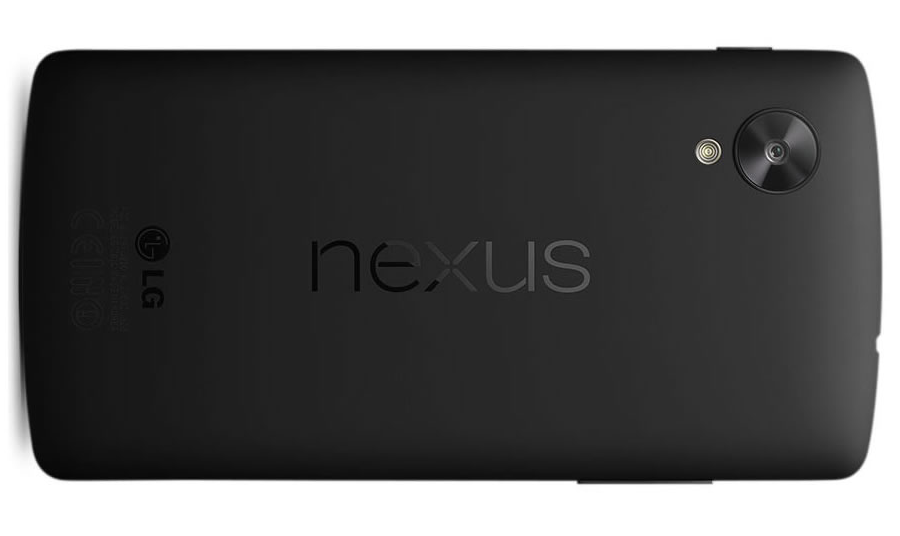
\includegraphics[width=\textwidth/3]{Bilder/Robot/nexus_backside}
\caption{Servo-Motor des NXT-Systems}
\label{fig:motor}
\end{figure}

